\chapter{Implementation}
Patients, physicians, and researchers do not only want to store OSA signal into a relational database system, but also want to do data analysis based on the collected data. Computing ability and storage capability of mobile devices are huge improved, and the users would like to store and perform data analysis on these devices. Therefore, a database system application on mobile platform for the designed database model in Chapter 4 needs to be taken into considering. The implementation mainly focuses on developing sensor wrappers on Android operative system for the designed database, and writing SQLite codes to do data analysis. Hence, other functions such as GUI interactions between users and the application, visualizing data on graph, etc., are minor. It is to say, not all of features are implemented, therefore, the implementation is a proof-of-concept. This chapter presents a traditional software engineering approach, in which, the waterfall process model approach is mainly used for developing the application. It is because the process activities can be separately presented (requirements specification, software design, implementation and so on). Incremental development approach is useful when the requirements changes frequently, and new functions need to be added to the previous version. Hence, it is not suitable for the OSA database system, since the data requirements are stable. At the time of the writing, the OSA data are not stored in any relational databases. Instead, each clinic has their own file format for storing the data. The users can either use the provided tools from these clinic, or ask for a general format file (EDF format) in order to do data analysis. Therefore, reuse-oriented software engineering approach cannot be used, since the database application must be developed from scratch than integrated into an exist system.\\
In this chapter, functional and non-functional requirements of the users are carefully analyzed. These requirements are presented in Section 5.1; they are supplementary to the discussed requirements in Chapter 4. Section 5.2 presents an abstract model of the database system application and architectural models with respect to real-time wrapper and EDF wrapper. Possible data mining algorithms are also discussed in this section. Section 5.3 presents an Android specific implementation of the discussed models and the implementation of possible data mining algorithms.
\section{Requirements for database application}
\begin{table}
\begin{adjustwidth}{-1.5cm}{}
\begin{center}
\begin{tabular}{ |p{2.4cm}|p{5.5cm}|p{3.3cm}|p{4.3cm}|}
 \hline
 User requirements definition& System functional requirements& System non-functional requirements& Structured specifications\\
 \hline
 The application must reuse CESAR acquisition tool to collect data from BITalino.&
 1. System must open a port for that CESAR acquisition tool can connect and send data.\newline
 2. System must follow CESAR package formats for that the data can be correctly collected.\newline
 3. System must let the users fill out the requirement fields for patient and clinic before storing a record into database system.\newline
 4. System must support multiple connections.&
 - Product: usability, performance, space, reliability\newline
 - Organization: Android operative system (6.0)\newline
 - External: must follow the protection of personal data of patient&
 - Input: metadata and data packages from CESAR\newline
 - Source: BITalino\newline
 - Output: store metadata and data to database system, and may plot them to graph\newline
 - Place: fragment server application and fragment real-time visualization\\
 \hline
 The application must support importing and exporting EDF files.&
 1. The user can freely choose a EDF file to import, and import progress must be showed.\newline
 2. The user can partially import an EDF file by click stop button, in case they do not want to wait.\newline
 3. System must support fully or partially export. That is, the user can choose from time – to time when exporting.\newline
 4. The user can choose which channels they want to export.&
 - Product: usability, performance, space, reliability\newline
 - Organization: Android operative system (6.0)\newline
 - External: must follow the protection of personal data of patient&
 - Input: EDF header and EDF data record\newline
 - Source: EDF file\newline
 - Output: store/export EDF header and data record to database system/EDF file\newline
 - Place: fragment EDF reader and fragment EDF exporter\\
 \hline
 Data analysis can be perform by using the application.&
 1. The system must support raw query, in which the users can write SQL queries to retrieve whatever they want.\newline
 2. The system must provide some mining functions to detect OSA signal.&
 - Product: usability, performance, space, reliability\newline
 - Organization: Android operative system (6.0), SQL query language&
 - Input: data in database system\newline
 - Source: database system\newline
 - Output: result from SQL, or OSA detection\newline
 - Place: mining fragment\\
 \hline
 Collected data could be visualized in real-time data, or replay from the stored data.&
 1. The user can visualize data on a graph view.\newline
 2. Channels can be freely choose to visualize to do comparison.&
 - Product: usability, performance, space, reliability\newline
 - Organization: Android operative system (6.0)&
 - Input: BITalino or database\newline
 - Source: BITalino or database\newline
 - Output: graphic view\newline
 - Place: fragment real-time/replay visualization\\
 \hline
 Annotations could be added manually to a certain source.&
 Annotations could be manually added and stored while visualizing sources.&
 - Product: usability, performance, space, reliability\newline
 - Organization: Android operative system (6.0)&
 - Input: data in database\newline
 - Source: database\newline
 - Output: annotations from users are stored in database system\newline
 - Place: fragment replay visualization\\
 \hline
\end{tabular}
\end{center}
\end{adjustwidth}
\caption{A summary of the database system application requirements}
\label{tab:userrequirementAPP}
\end{table}
This section presents and analyzes the specific requirements of the users as well as the database application system. The analysis results provide the foundation for designing the data model and the implementation for the application.\\
User requirements are usually presented as statements. These statements are in natural language, and are about services that the system is expected to provide to the users, and constrains for the services. On the other hands, system requirements present a list of system requirement specifications for each user requirement statement. In short, the users define the requirements, while the system specifies in detailed the services it provides, inputs and outputs, functional and non-functional requirements, etc., for each of defined requirement.\\
Functional requirements are statements of services the system should provide, how the system should react to particular inputs, and how the system should behave in particular situation \cite{INF1050BOOK}. On the other hands, non-functional requirement are constraints on the services or functions offered by the system. They are included timing constrains, constrains on the development process, and constraints imposed by standards \cite{INF1050BOOK}.
Table \ref{tab:userrequirementAPP} presents the requirements of the database system application. In which, each user requirement defines the services the system must provide. Correspondingly, the system requirements clearly explain how the system must behave to satisfy the user requirement. These system requirements are presented in forms of functional requirements and non-functional requirements, and structured specifications of the requirements. “Place” in structure specifications column presents which function groups the requirements belong to. By grouping requirements in a group of functions, it is easier to design and implement. Function groups are illustrated in Figure \ref{fig:Figures/OSADBSContext}.
\begin{figure}[ht]
    \centering
    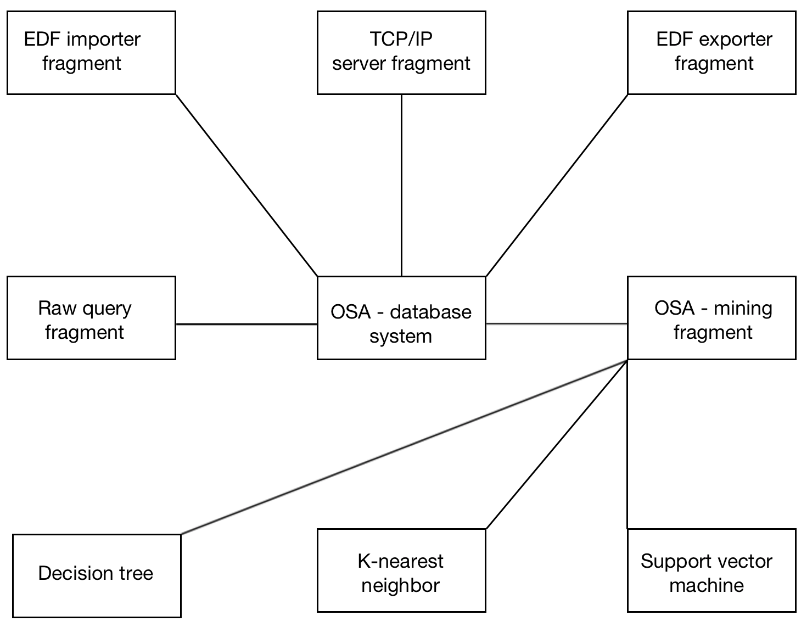
\includegraphics[width=1.0\textwidth]{Figures/OSADBSContext.png}
    \caption{The context of the OSA database system application}
    \label{fig:Figures/OSADBSContext}
\end{figure}
The first two and the last three requirements in Table \ref{tab:userrequirementAPP} are respectively corresponded to “what it must contain” and “what the database is to be used for” presented in the database modeling chapter. In other words, the database application needs to be implemented two wrappers that collect data from CESAR acquisition tool and EDF/EDF+ file formats, then the collected data can be used for analyzing, visualizing, or modifying. Since the mainly focus of the thesis are collecting data and data analysis, therefore visualizing and modifying are added as helper functions.\\
The first two user requirements illustrate that the system must support collecting samples from BITalino by using CESAR acquisition tool, and importing EDF/EDF+ data. As presented in Chapter 3, for collecting samples from CESAR acquisition tool, the system first establishes a TCP/IP connection to the tool, then the metadata and data packages are sent to the system. The structure of these packages are well documented, and have been discussed in Chapter 3. The user can also use multiple acquisition tools to collect sample, hence the application must support multiple connections as well. Since CESAR acquisition tool does not send the information of the clinic and patient, the information must be manually filled by the user before recording samples. CESAR acquisition tool provides data in real-time, therefore the system must operate with respect to the given non-functional requirements presented in Table \ref{tab:userrequirementAPP}. Likewise, for importing and exporting EDF/EDF+ files, the system must follow the structure of the EDF/EDF files which are also well discussed in Chapter 3. Since the files can be very large, the system must satisfy the non-functional requirements when importing and exporting.\\
As mentioned earlier, visualizing and modifying are not the main focus of the thesis. They are added to the database system application as helper functions to help the user have a better view on the collected data. Therefore, they are implemented as proof-of-concept and “enough for using”. For the analysis requirements, a raw query function is useful when analyzing the data. However, in term of security, this is quiet dangerous action. In the top 10 vulnerabilities, SQL injection stands on the top of the list\cite{OWASP}. In this case, the risk does not come from stealing of sensitive information, or compromising the database. It is dangerous if the researchers accidentally perform queries that can result the database system corrupted, such as deleting a column in a data table, drop a table, etc. Filter out vulnerable queries is a topic for researchers who are interested in database security. Hence, to filter out vulnerable queries is not in scope of the thesis. An assumption is made that the users have the knowledge on database system, and they do not perform any vulnerable queries. The system must also provide some of possible mining algorithms that are used for detecting OSA signal.
\section{Database application modeling}
As presented in Figure \ref{tab:userrequirementAPP}, the context of the OSA database system consists of importing, exporting and analyzing data. Data sources, in which the system collects data from, can be divided into two groups. Sources that connect to the database system via TCP/IP protocol are real-time sources. On the other hands, non-real-time sources are from EDF/EDF+ files. Data analysis are only performed on the stored data. Currently, the system does not support real-time analysis, since the goals of the system are collecting raw data for future analysis. That is, the collected data are used as the inputs for many different analysis algorithms than the possible mining methods presented in this thesis. However, real-time OSA data analysis is good to be considered, and an exciting topic for researchers who are interested in online analytical processing.\\
Subsection 5.2.1 presents real-time wrapper modeling, in which, some real-time attributes are taken into considered, and how the TCP/IP server fragment is modeled. Subsection 5.2.2 presents the modeling for non-real-time wrapper, in which EDF importer fragment and EDF exporter fragment are carefully modelled.
\subsection{Real-time wrapper}
When choosing the appropriate real time sensor sources, several factors should be considered, such as the quality of signal, mobility, how many channels can it observe, which protocol it uses to send data sample, etc. The BITalino platform is chosen as sensor source after carefully considering the pros and cons of it in Chapter 3.\\
In terms of real-time data stream source, the system has to deal with data stream management problems. The thesis targets at a solution to store the OSA bio-signals, and it does not address data stream management system issues, where the queries need to be apply on the data stream. Instead, some general real time factors need to be seriously considered when designing the database system. These factors are arrival rate, timestamp, physical resource, one-time read data, data stale or imprecise, and unpredictable data arrival. When the incoming rate is high, it might be a problem to store all the data, because of the limitation of the mobile platform. Even on a stationary computer, storing data streams could be a problem and needs to be considered.\\
To choose a suitable solution for manage the arrival rate of the data stream, it is good to review and discuss how the data stream management system (DSMS) deal with real-time data stream problems. Due to the unboundedness of the data stream, it is essential to capture the stream into small slices which is called windows. To manage the data stream, DSMS uses window models, in which the models are based on the direction of movement of the endpoints, that are fixed window, sliding window, and landmark window. As the name of the window models, the fixed window has a fixed amount of samples or time interval. The sliding window contains the data from now up to a certain range in the past. The landmark window, on the other hand, contains the data from the beginning until now. The window size can be either physical/time-based or logical/count based. Figure \ref{fig:Figures/windows} presents an overview of the fixed window and sliding window.
\begin{figure}[ht]
    \centering
    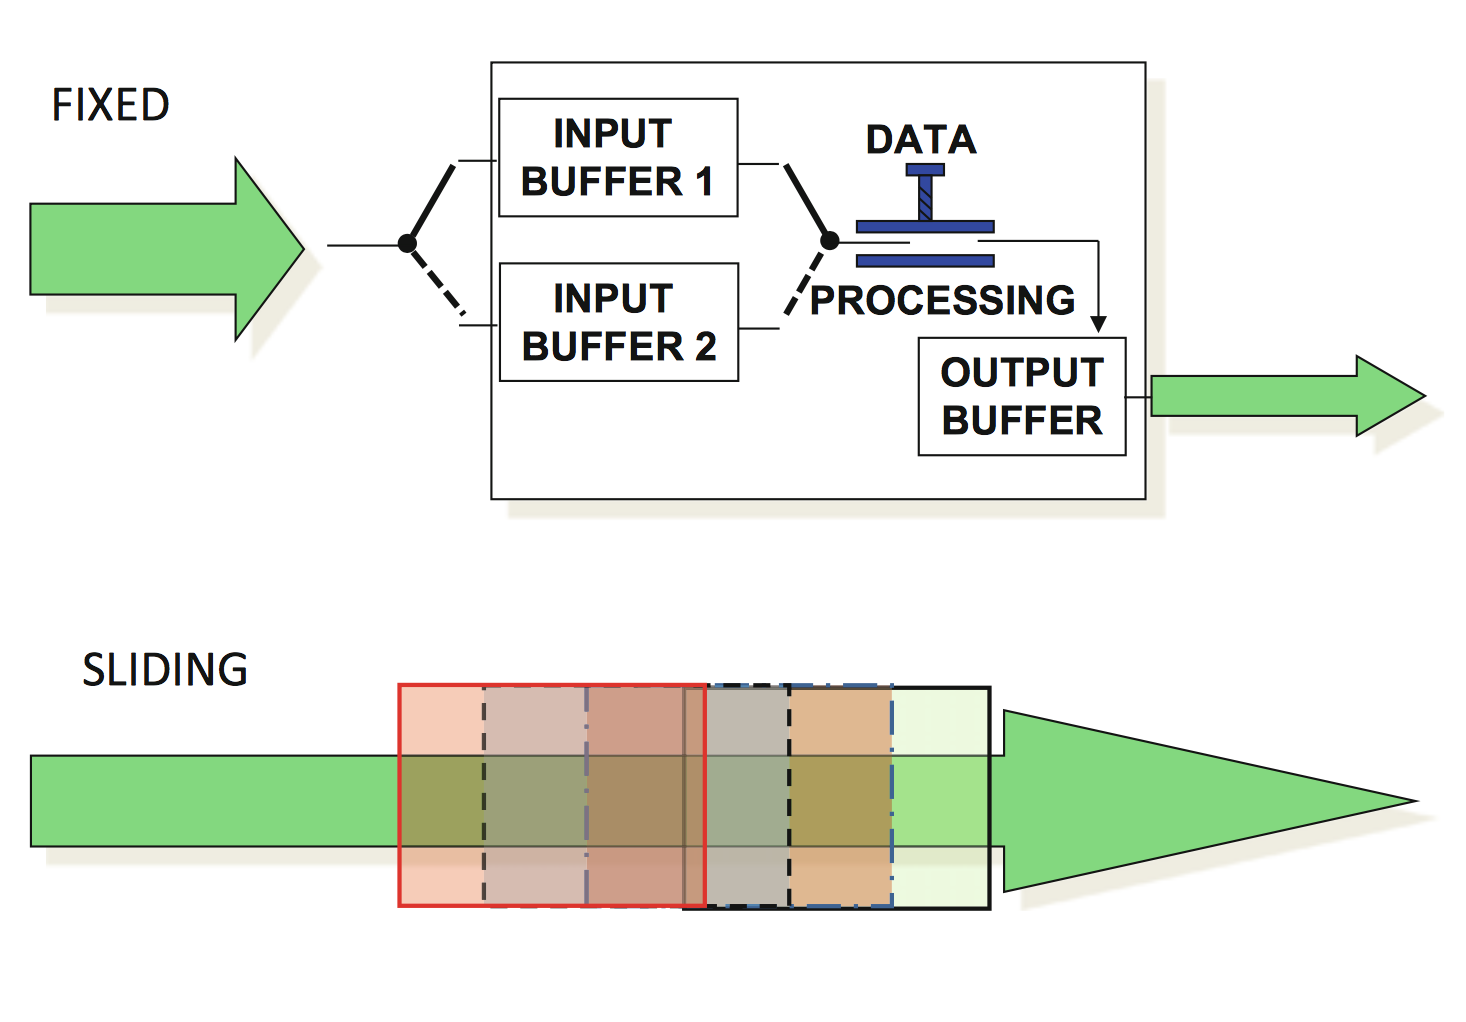
\includegraphics[width=0.6\textwidth]{Figures/WINDOWDSMS.png}
    \caption{Example of fixed and sliding windows \cite{DSMS_WINDOW}}
    \label{fig:Figures/windows}
\end{figure}
When a sample arrives, it is updated either immediately (eager processing) or when the window is full (lazy/batch processing).\\
Tasks of the system are to store the raw data samples as well as to display these samples to a graph view with respect to the users’ requirements. To ensure that the tasks are well performed, the system uses two buffers which functioned as windows in DSMS. It is to say, the first buffer is a fixed window, count based, and batch processing, that is used for collecting samples for the database. The second buffer is a sliding window, count (or time) based, eager processing, that is used for collecting samples for graphic view. By using these two buffer, the system ensures that the overhead of writing to database is minimized (by using batching processing), while the performance increases (by using eager processing).\\
If the order of the samples plays an important role for later analysis, the timestamp must be explicit (timestamp from data source). Otherwise, the implicit timestamp (system time) can be used. The CESAR acquisition tool provides the timestamp in each sample object. However, the timestamp is pre-converted and need to be handled before using for plot view. It is an overhead for converting timestamp for each sample. However, there is quite easy to change some code in the acquisition tool for that the can send a raw timestamp (Unix timestamp). Therefore, the explicit timestamp is considered a better solution than the implicit timestamp with respect to the accuracy of the arrival samples.\\\\
\textbf{Server thread}\\
The collector of CESAR acquisition tool offers two methods for that the database application can collect data from it. The collector can either save data to a text file or send them to a given server IP and port address by using TCP/IP protocol. Since the database system application wants to have real-time data from BITalino, it must open a port to collect data. As presented in requirement section, the system must support multiple connections, because the user may use multiple sensor source to monitor the body. Therefore, multiple threads system must be implemented. Each thread manages one sensor source. The main thread therefore just waits for connections, creates and hands in necessary information to the new created thread, then starts the new thread. The main thread must have a way to manage the created threads for that the users can choose a source they want to interact with from the connected list. A Unified Modeling Language (UML) activity diagram is used for illustrating how the main thread works as presented in Figure \ref{fig:Figures/ServerActivity}. UML is a famous and widely used modeling language, however, a short explanation on the used annotations is needed to make the figures easier to understand. In UML activity diagram, a filled circles indicates the start of a process. Activities are presented by rectangles with round corners. Arrows present the flow of work between activities. Annotations on the arrow indicate the condition when the work flow is taken. A filled circle inside another circle indicates the end of the process.\\
\begin{figure}[ht]
    \centering
    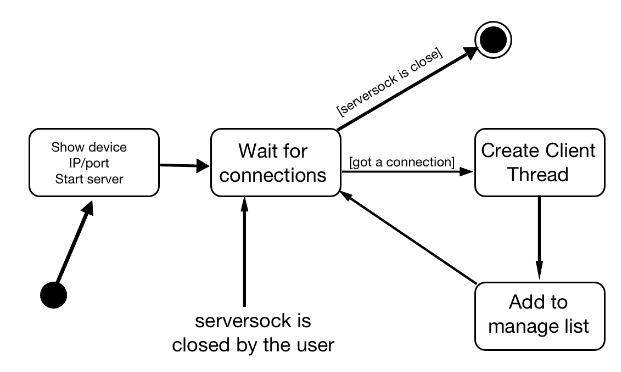
\includegraphics[width=1.0\textwidth]{Figures/ServerActivity.png}
    \caption{Process model of server thread}
    \label{fig:Figures/ServerActivity}
\end{figure}
\textbf{Client thread}\\
Most of the jobs of the wrapper are handled in the client thread. Once a client thread is created, it waits for arrival data, then pushes to database or adds to graphical view if these actions are flagged. Data packages from CESAR acquisition tool are well discussed in Chapter 3, in which a metadata package is sent first to identify the sensor source, then the source keeps sending its data via the connection between the database system application and the acquisition tool. As explained in the real-time characteristics, the client thread must share two buffers with the other threads. The first buffer is used for storing samples to the database, and the second buffer is used for showing samples on a graphic view. However, these buffers are initialized only if the corresponded flags are flagged. That is, arrival samples are thrown if the users do not want to store or visualize them. Figure \ref{fig:Figures/ClientThreadAc} presents a possible implementation of the client thread by using a UML activity diagram.
\begin{figure}[ht]
    \centering
    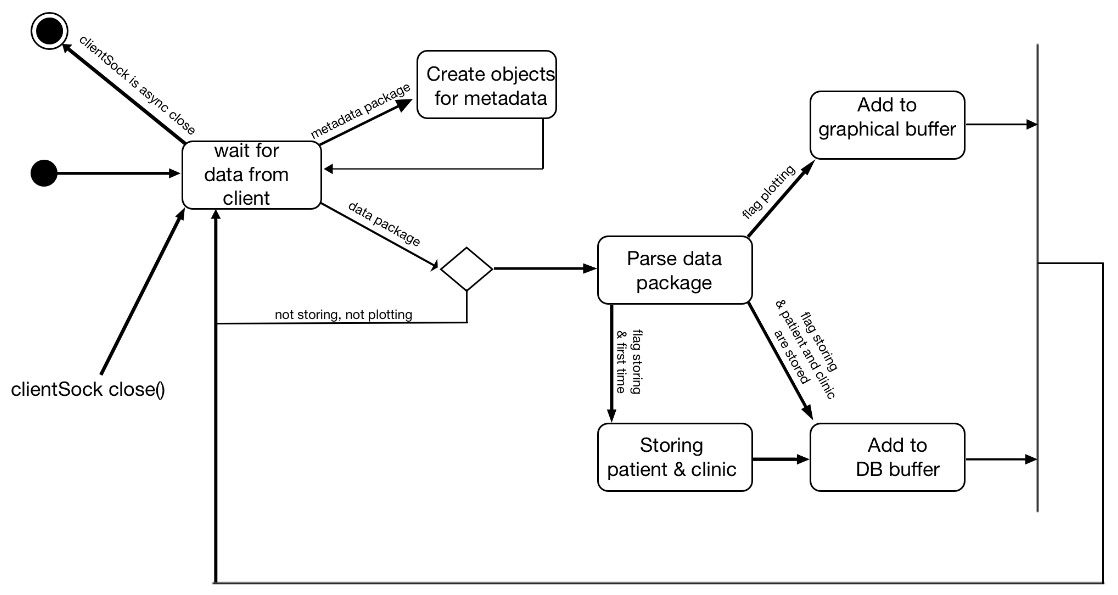
\includegraphics[width=1.0\textwidth]{Figures/ClientThreadAc.png}
    \caption{Process model of client thread}
    \label{fig:Figures/ClientThreadAc}
\end{figure}
As illustrated in the requirements, the system must be reliable and have a good performance. That is, no samples data are lost under recording, and the visualization must not be frozen. To satisfy these requirements, two different buffer management methods are used. A buffer, which is used for storing samples, maintains a list of fixed number of samples (it is to say, a record fragment), and a thread. The thread takes a full record fragment to store into the database, or waits for available record fragments if the list is empty. Since SQLite can perform about 50,000\cite{SQLITEORG_INSERT} insert statements per second, while the maximum number of samples BITalino can delivery is 1000 samples per second (1000Hz), the algorithm for this buffer is therefore satisfied the non-functional requirement (reliable). The second buffer can be implemented by using the algorithm from Producer and Consumer problem, in which the client thread is the producer, and a thread that update the graphic view is the consumer. However, this buffer is used as a sliding window, therefore a simpler solution can be used. That is, each time client thread adds a sample to a buffer list, it removes the oldest sample if the buffer is full. After that, a graphic view thread is notified to refresh the plot view.\\
Figure \ref{fig:Figures/ThreadsDBPlot} presents how the sever thread, client thread, database, and graphic view connect to each other’s.
\begin{figure}[ht]
    \centering
    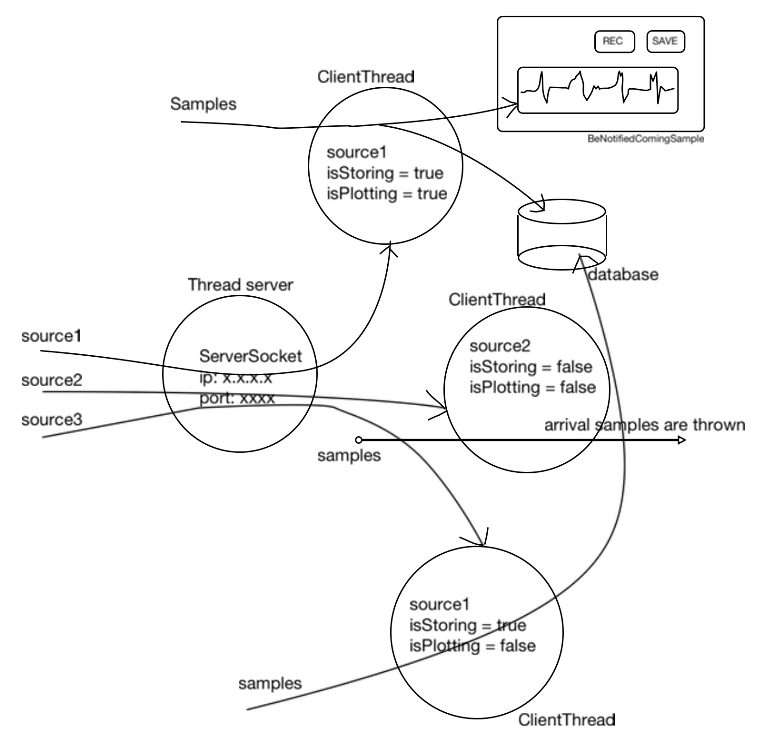
\includegraphics[width=1.0\textwidth]{Figures/ThreadsDBPlot.png}
    \caption{High level design of real-time wrapper}
    \label{fig:Figures/ThreadsDBPlot}
\end{figure}
\subsection{Non real-time wrapper}
Diverse data sources are essential in research. Using multiple sources of data in research often produces more accurate results and more objective values than using a single data source. There are many trustworthy sources that can be used for OSA data analysis. One of the sources that is chosen in this thesis are the Physionet sensor databases, which have been described in Section 3.1.2. The other non-real time source that the system collects data from, is NOX-T3 sensor source system. Theoretically, this source can be used as a real time sensor source. Although Nox-medical has an Android application, which is only support NOX-A1-PSG at the time of this writing, to collect samples from their devices, the NOX-T3 device neither provide any API for mobile platform, nor any documents that describe how to collect samples from the device as BITalino does. As mentioned earlier, it is very difficult to manage diverse sources when they have their own format. Fortunately, the problem is solved by using an EDF or an EDF+ file format to share data between source owners. The formats are fully described in Section 3.2.2 with respect to why they are introduced, what information these file contain, and how to use them. Therefore, the system is designed in the way that is opened for all of the sensor sources, as long as these sources can export their data to an EDF or EDF+ file format. In other words, the system only accepts source files in EDF form.\\
An EDF file can be very large, and can excess the main memory size. Hence, to satisfy the performance and robustness, the system should neither keep all the data in memory, nor call the database insert function for each sample. The problem could be solved by using the idea from real time sensor source. In other words, the system uses the concept of a window model, lazy update (batch processing) to solve the memory problem with the non-real time source.\\
Physionet databases and NOX-T3 sensor source can be used as non-real-time sources, because both of them provide a function to export their bio-signal data to EDF. “mit2edf” is a function from physiotools provided by Physionet. This function is used for converting between EDF and WFDB-compatible formats. NOX-T3 provides a graphic, step by step, and user friendly way to export their data to EDF.
\subsubsection{EDF importer}
As introduced in Chapter 3, EDF is one of the standardized data formats for bio-signals that used for storing and exchanging multichannel biological and physical signals. There is many tools and open source codes which can be used for reading a EDF file. Different tools have different goals when reading the EDF file. Most of them parse the samples to a graphical view and an annotations list, the others try to convert samples into text files that contain information for each channel and the record. EDF browser and EDF library\cite{EDFLIB} are one of the most famous used tools to view and parse EDF files. The performance of the tools is quite good since they are written in C code. Another open source tool that can be used for parsing EDF files to text files is Java-parser for EDF format\cite{EDF4J}. As the tool named, it is written in Java code, hence, the performance when parsing EDF file is poorer compared with EDF library. Since EDF/EDF+ file formats are well documented, it is easy to write a parsing tool. As discussed, different tools have different purposes when parsing EDF files. Since the one of the main goals of EDF file format is used for exchanging biological data, the EDF files need to be parsed into the received system data structure. Many parsers try to load the whole EDF file into main memory before converting. As discussed, the EDF file can be extremely large, the parsers therefore crash; Java-parser for EDF format is one them.\\
There is no need to “reinventing the wheel” rather using them in a smart way. Since in the designed database system, each bio-object is stored in a separate table. Therefore, the EDF importer can use the functions in an EDF library to read the EDF files. The information, which are read from EDF, are stored into the corresponded tables. In case the used library tries to read the whole EDF file into memory, an optimization, which is multiphase read, need to be used. Figure \ref{fig:Figures/EDFImporter} presents a UML activity diagram which explains how a EDF file can be read into the database without memory problem.
\begin{figure}[ht]
    \centering
    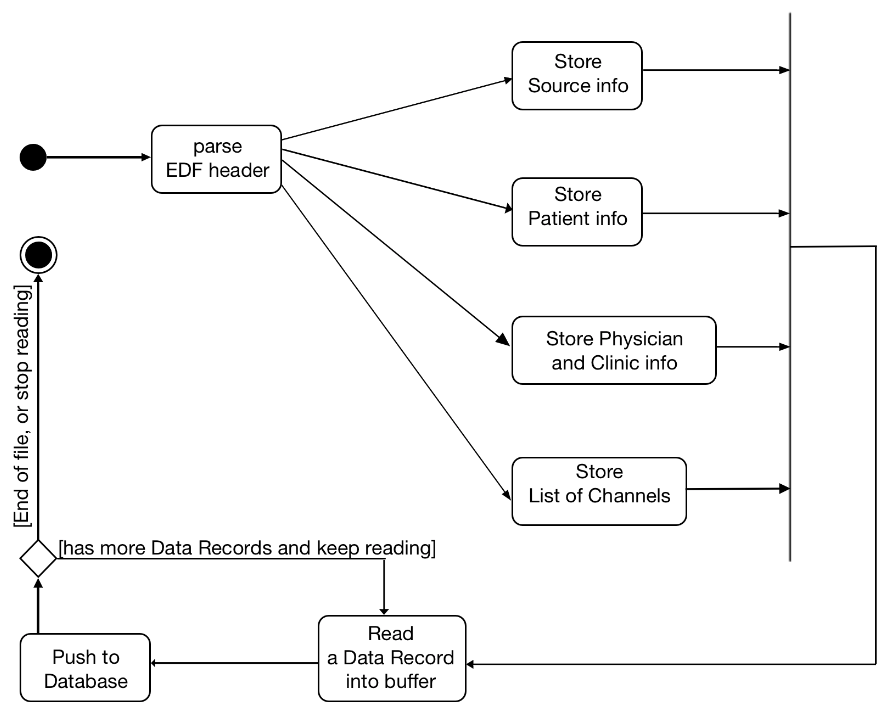
\includegraphics[width=1.0\textwidth]{Figures/EDFImporter.png}
    \caption{Process model of EDF importer}
    \label{fig:Figures/EDFImporter}
\end{figure}
\subsubsection{EDF exporter}
Sharing data is essential in researching. Therefore, the system must export its data into a standardized data formats for bio-signals, a EDF file. On the other hands, the system targets to be implemented on a mobile platform, where resources are very limited. Exporting data and saving it in external storage places is vital to satisfy non-functional requirements, where the collected data must not be lost when the storage capability of the mobile devices exceed. There is no need to export the whole source of data to a EDF file, some of channels or samples are exported for special needs. For example, there is a project, in which researchers or physicians need only samples from ECG channel, it does not make sense if the EDF file contains samples for the other non-relevant channels. Furthermore, if a project needs to analyze all samples which collected on nighttime, the added daytime samples are waste of not only the storage, but also time to parse the EDF file when using. Therefore, the system must let the users choose which channels and periods they want to export. As discussed in the non-functional requirements for EDF importer and exporter, the information of the patient must follow the protection of personal data law. That is, the patient must be exported as anonymous, otherwise there must be an agreement of the patient. Figure \ref{fig:Figures/EDFExporter} is a UML activity diagram that illustrate how data are exported into a EDF file.
\begin{figure}[ht]
    \centering
    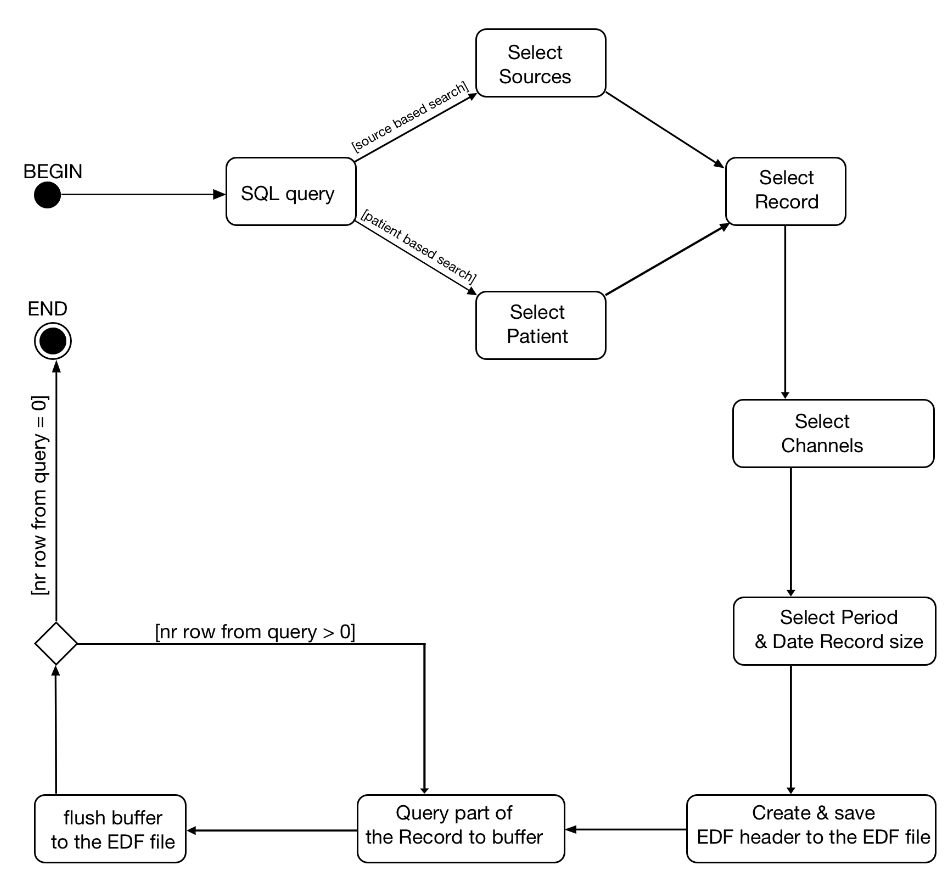
\includegraphics[width=1.0\textwidth]{Figures/EDFExporter.png}
    \caption{Process model of EDF exporter}
    \label{fig:Figures/EDFExporter}
\end{figure}
\section{Database application implementation}
Based on the database and the database application modeling, a chosen software platform must be operated on mobile devices, and must support features that the designs require. Both Android and iOS operative system are the good candidates for the position. They all support threads, SQLite, TCP/IP connection, Bluetooth, etc. However, there is difficult to say which one is better, it depends on the user favorites. Since the implementation is a proof-of-concept, it is no need to deeply argue why choosing iOS or Android as long as they meet the requirements. Android platform is chosen for the designs in the thesis for some reasons. First of all, according to netmarketshare.com\cite{NETMARKETSHARE}, there is 66.71\% devices installed Android operative system compared to 29.55\% devices installed iOS. Moreover, applications for Android are written by using Java programming language, which is very easy to be read and understood by many developers. Nonetheless, it is easy to synchronize and test with CESAR acquisition tool, because the tool is written for Android.
Beside satisfying the function and non-function requirements, the implementation also focuses on the graphic user interface (GUI). It is natural that people have a better feeling when they interact with icons and symbols compared to text. By using GUI, the system can avoid asking input from users, instead it lets the users choose via provided input or default values, because typing text on a mobile platform is a cumbersome task.\\
Subsection 5.3.1 presents a short discussion on how to manage multi-threaded database accessing in SQLite database system on Android platform. Subsection 5.3.2 presents how to implement the real-time wrapper model on the chosen platform for collecting data from CESAR acquisition tool. Subsection 5.3.3 presents the implementation of non-real-time wrapper, in which the EDF import and export functions are implemented accordingly to the abstract designs in Subsection 5.2.2. Subsection 5.3.4 presents a simple implementation, in which the collected data can be visualized on a graphical graph view.
\subsection{SQLite and Multi-threaded database accessing}
In SQLite, the same database can be shared by multiple processes at the same time. By using read/write locks, SQLite can control the ways processes accessing to the database. The processes can perform read operations at the same time, but only one process performs write operations at any moment in time. From version 3.5.0, SQLite manage locks internally to avoid data corruption. Hence, several threads can use a single SQLite connection simultaneously. That is, the application does not need to manage the database accessing between threads. However, balancing database workloads between threads need to be considered, it is because when any thread wants to write to the database, it locks the entire database file for the time it uses for writing.
A statistic on the relative number of devices running a given version of the Android platform from Google presents that more than 99,9\% devices running an Android version with API 10 or better \cite{DEVELOPERANDROIDAPI}. According to the dependence between Android API and SQLite version\cite{DEVELOPERANDROIDSQL}, SQLite 3.6 comes with Android API 8; the higher the Android API is, the better SQLite version it has. Therefore, most of current mobile phones have the SQLite version better than 3.6 which supports the internal database-level locks to avoid database corruption. However, database accessing can be failed if each process has its own connection to the database file. It is because the SQLite does not support synchronization between multiple connections. When one connection is in use for writing, the database rejects the other modifying activities from other connections. As a result, the database management does not update changes of the other connections. To use multiple threads for maximizing database performance is not benefited, since there is only one modifying connection at a specific time.\\
Threads can be used to maintain a shared connection for different data sources, or different data using purposes. These threads take turn using the database connection. By sharing the connection, the application makes sure that all threads can correctly update their data into the database. In the thesis, a helper object OSADataBaseManager is implemented in a way it is transparent for threads who using it. That is, a thread can initialize an instance of the object, then it can get the SQLiteDatabase via the openDatabase() method of the instance. After doing database operations, the thread can ask the instance for closing the database connection. At the view of the thread, it is logic when the thread open database connection for doing some tasks, then close the connection. However, the OSADataBaseManager instance creates and maintains only one SQLiteDatabase connection for all threads. The connection is created whenever there is at least one thread want to connect to the database, and closed when there are no database requests. Listing \ref{listing:SQLiteConnection} presents how to manage the shared database connection when working with multi-threaded database access.
\begin{code}[ht]
\begin{lstlisting}
    private int mOpenCounter;
	private static OSADataBaseManager instance;
	private static OSADBHelper mOSADBHelper;
	private SQLiteDatabase mDatabase;

	public static synchronized void initializeInstance(OSADBHelper helper) {
	    if (instance == null) {
	        instance = new OSADataBaseManager();
	        mOSADBHelper = helper;
	    }
	}

	public static synchronized OSADataBaseManager getInstance() throws Exception{
	    if (instance == null) {
	        throw new Exception(OSADataBaseManager.class.getSimpleName() 
	                + " call initializeInstance(..) to initialize instance.");
	    }
	    return instance;
	}

	public synchronized SQLiteDatabase openDatabase() {
	    mOpenCounter++;
	    //If it is the first time
	    if(mOpenCounter == 1) {
	        mDatabase = mOSADBHelper.getWritableDatabase();
	    }
	    //else just return the opened instance
	    return mDatabase;
	}

	public synchronized void closeDatabase() {
	    //We do not want to close the DB while the other use it
	    mOpenCounter--;
	    if(mOpenCounter == 0) {
	        //REAL CLOSE
	        mDatabase.close();
	    }
	}
\end{lstlisting}
\caption[SQLite connection management]{SQLite connection management}
\label{listing:SQLiteConnection}
\end{code}
\subsection{CESAR wrapper}
As presented in the high level design of real-time wrapper, the wrapper must implement two kinds of threads. The first one is used for maintaining a list of connected sources that not only from CESAR acquisition tool, but also from other acquisition tools, as long as the sources follow the package interfaces that are discussed in Chapter 3. The second one is used for maintaining the connection between the application and a certain sensor source. Figure \ref{fig:Figures/CESARGUIWrapper} presents the GUI of the wrapper. 
\begin{figure}
    \centering
    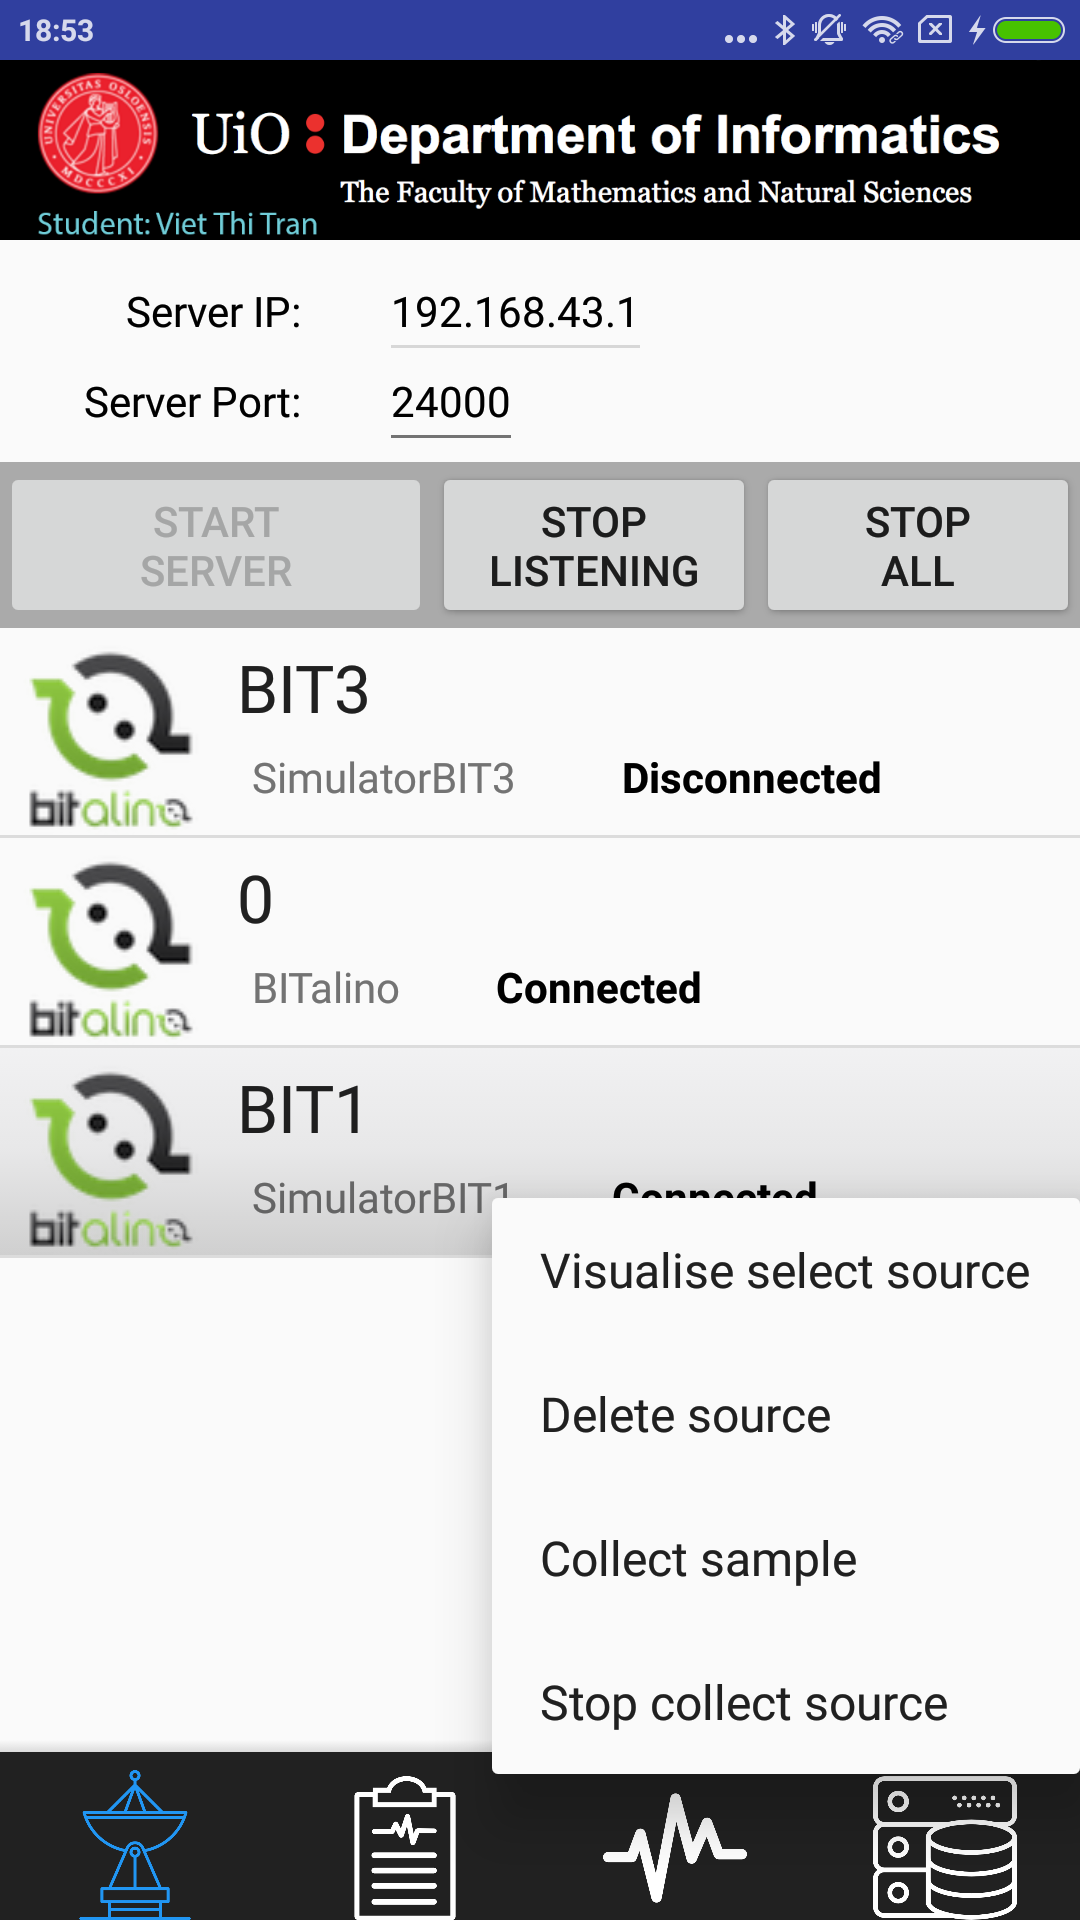
\includegraphics[width=0.4\textwidth]{Figures/CESARGUIWrapper.png}
    \caption{Graphic user interface of the wrapper for CESAR acquisition tool}
    \label{fig:Figures/CESARGUIWrapper}
\end{figure}
In the figure, the application provides the IP number and the port it listens to. There are two active sources (with status “connected”) and one inactive source (with status “disconnected”) in the figure. By long clicking on a source, a list of functions, which the user can interact with, is showed. Each component that is presented in the figure is equivalent to a function the wrapper need to provide. The functions are divided into two groups; the first group consists of starting server, stopping listening, stopping all client threads and disconnect the server, managing the current connected list, and providing functions for that users can interact with the current connected list. These functions belong to server thread which is implemented in \textbf{ServerFragment.java} in the implementation code. The second group consists of collecting data from a specific source, forwarding data to graphical view (if requested), managing a batch processing for storing data into the database; these functions belong to client management thread which is implemented in \textbf{ClientThread.java}.\\
\textbf{ServerFragment.java}
As Figure \ref{fig:Figures/ServerActivity} in abstraction level design presented, the application must get the IP address of the device and show it on GUI. It can be done by checking all the network interface devices, and finding the IPv4 from the interfaces. Users are freely to choose a port number which must be bigger than 1024, it is because port smaller than 1024 are system ports\cite{IANAPORT}. To make it easy for the user, a default port is provided before the application is started. Once everything is initialized, the user can click on “START SERVER” button to begin the listening process, which waiting for sensor sources at the presented address and port number. When the user clicks on the “START SERVER” button, the button is disabled, and a server thread is created. The procedure when the button is clicked is illustrated as following:
\begin{adjustwidth}{1cm}{}
	server = new ServerSocket(portNr);\\
		loop:\\
	1.  wait for connections from clients; if get connection, go to Step 2\\
	2.  create a ClientTread object with necessary parameters\\
	3.  add the ClientThread into the managing list\\
	4.  start the thread and go to Step 1\\
		if server socket is closed (by clicking either “STOP LISTENING” or “STOP ALL” buttons), the server is shutdown, and the “START SERVER” button is enabled.\\
\end{adjustwidth}
Listing \ref{listing:ServerManagement} presents how the abstract design and the procedure are translated into coding in Android. With respect to GUI, "Toast" is used for posting a notification such that the user knows some events have happened. Other logics and codes for managing GUI are not the main focuses of the thesis, and therefore not to be deeply discussed in the writing. These codes can be found in the included project folder.
\begin{code}[ht]
\begin{lstlisting}
serverPort = Integer.parseInt(txtServerPort.getText().toString());
final Context CONTEXT = getContext();
Thread server = new Thread(new Runnable() {
	@Override
	public void run() {
	    try {
	        //Create a server socket object, bind it to server_port
	        sockServer = new ServerSocket(serverPort);
	        //Multi clients management
	        while (true) {
	        //Accept the client connection, then give it to ServerThread with client socket
	            Socket socClient = sockServer.accept();
	            final String clientIP = socClient.getRemoteSocketAddress().toString();
	            serverUpdateUI.post(new Runnable() {
	                @Override
	                public void run() {
	                    Toast.makeText(CONTEXT,"Got connect from: "
	                    +clientIP,Toast.LENGTH_SHORT).show();
	                }
	            });
	            ClientThread clientConnected = new 
	                         ClientThread(socClient,CONTEXT,serverUpdateUI, selv);
	            addNewSource(clientConnected);
	            clientConnected.start();
	        }
	    } catch (IOException e) {
	        serverUpdateUI.post(new Runnable() {
	            @Override
	            public void run() {
	                Toast.makeText(getContext(),
	                "SERVER IS SHUT DOWN",Toast.LENGTH_SHORT).show();
	            }
	        });
	        //WHEN sockServer close, it will be here
	        sockServer = null;
	    }
	}
	});
startServer.setEnabled(false);
stopListening.setEnabled(true);
stopAll.setEnabled(true);
server.start();
\end{lstlisting}
\caption[Server management]{Server management}
\label{listing:ServerManagement}
\end{code}
For each of sensor source in the connected list, the user can interact with the connected source via four provided functions, that are collecting sample, stopping collecting sample, visualizing, and delete the source from the list. With visualizing, if the source is not fully initialized, or disconnected, the user is not allowed to view the source. Otherwise, the application disconnects all client threads from the graphical graph, then connects the selected source to the graphical graph. It is because the graphical graph allows only one source to be visualized at a specific time. Any optimizations for the graphical graph are considered future works, since the thesis mainly focus on database and wrapper implementations. On the other hand, if the user clicks on “Delete source”, the application double checks if the user really want to delete the source from the connected list. If it is a case, the selected source is forced to be disconnected, and is removed from the managing list. If it is collecting data for the database, all the data in the buffer must be flushed into the database to ensure that no data losing under collecting process.\\
\begin{figure}
    \centering
    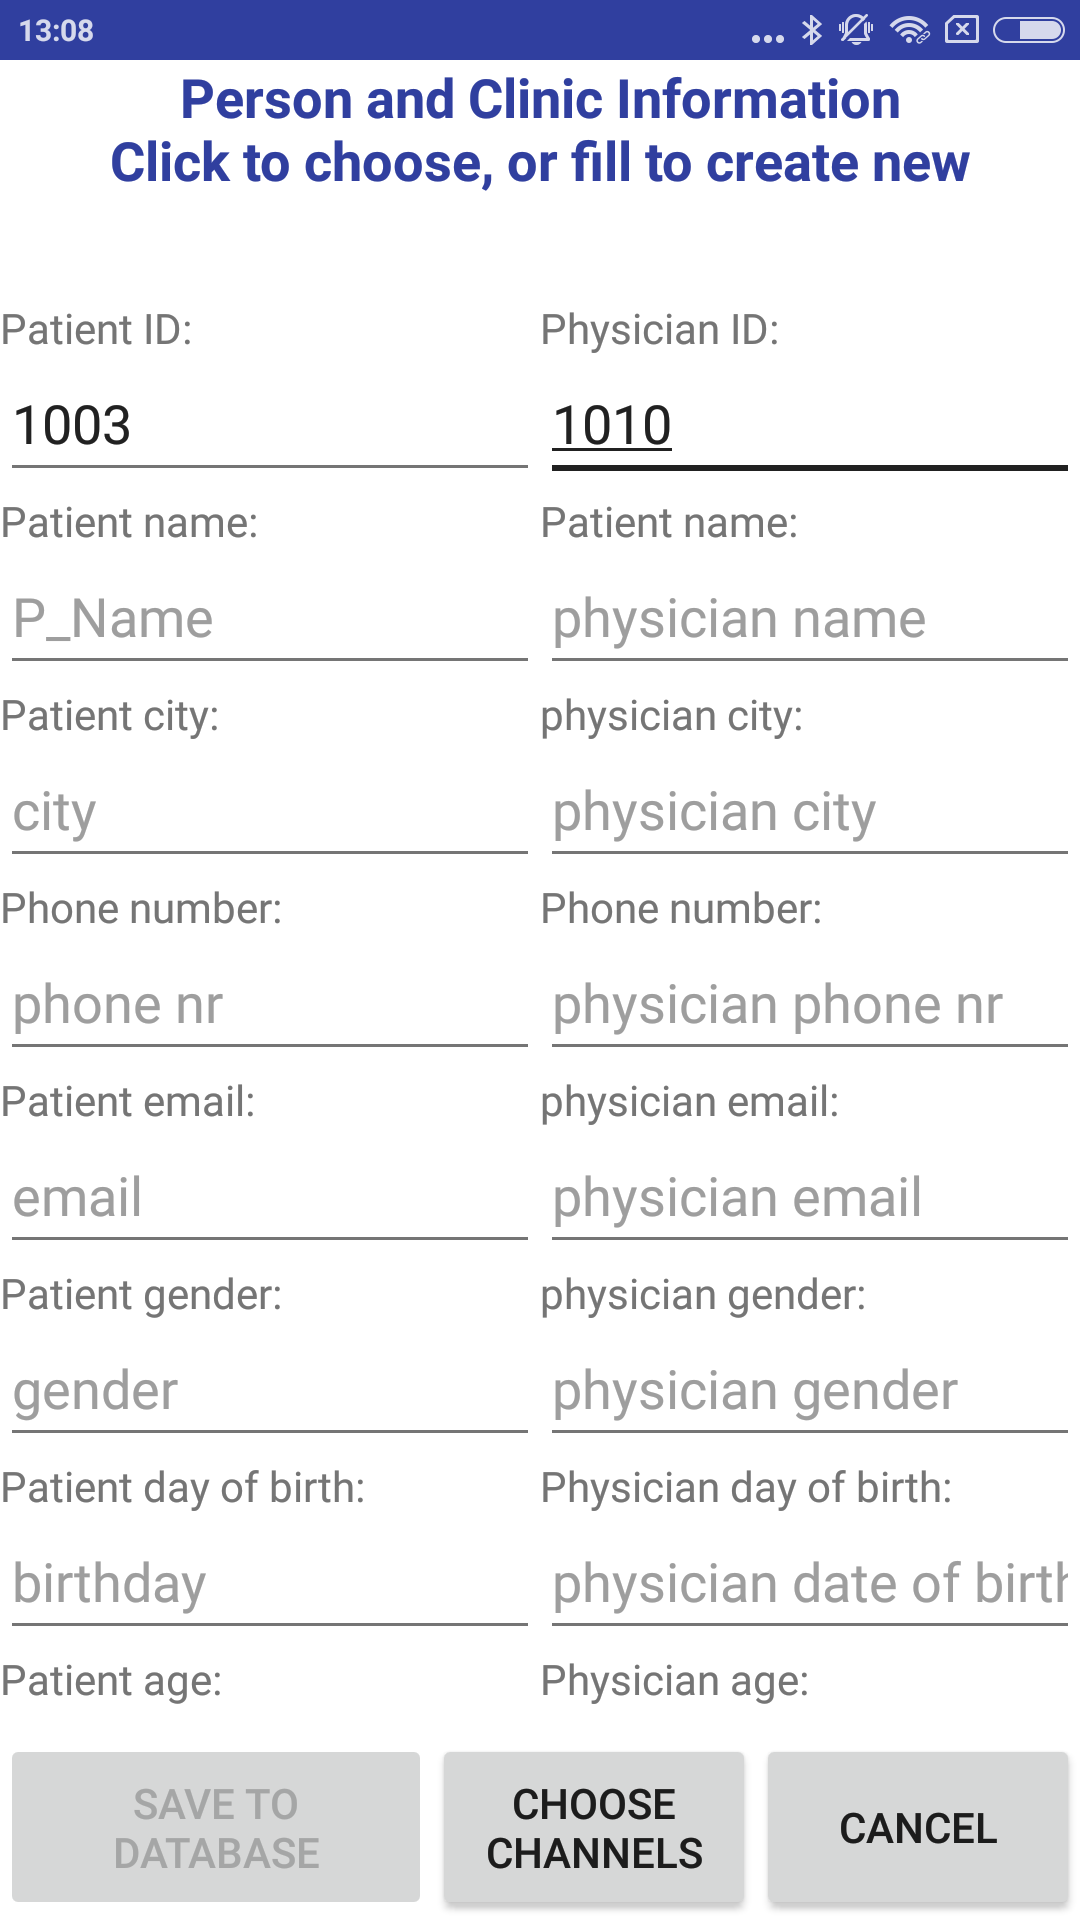
\includegraphics[width=0.4\textwidth]{Figures/clinicpatient.png}
    \caption{Form for getting user input for Patient, Physician, and Clinic}
    \label{fig:Figures/clinicpatient}
\end{figure}
The user can perform data collection on the sources with “connected” status. By clicking on one of them, the user is asked for the information for filling patient, physician and clinic information as presented in Figure \ref{fig:Figures/clinicpatient}. Since the patients are freely to choose the information they want to save, the fields in the form can be empty. However, the database need some information to manage the patient, physician and clinic, the user must at least provide information for the ID-fields. After that, the user must choose which channels to be stored, then by clicking on “SAVE TO DATABASE” button, the connected source is flagged as storing, and storing process is started. Stopping collecting is quite easy to implement, it can be done by flagging the selected thread as not storing, and ask the thread to flush the buffer into the database.\\
\textbf{ClientThread.java}
After a client thread is created, it immediately listeners for the incoming data at the input stream from its socket. As presented in Chapter 3, CESAR separates the sending data packages by using a newline character. The thread can get the arrival packages by calling readLine() on the input stream. For each line from the stream, the thread can parse the line into a JSON object, and the collecting process is initialized if the “type” of the object is “metadata”. Otherwise, the object is sent to graphical graph and the database if “isPlotting” and “isStoring” are flagged. The UML activity diagram from Figure \ref{fig:Figures/ClientThreadAc} in the high level design can be translated into specific implementation as following:
\begin{adjustwidth}{1cm}{}
	BufferedReader bf = get input stream from client socket;\\
	Loop: as long as the client thread is not disconnected\\
		1.  read a line from bf\\
		2.  parse the line to JSON object\\
		3.  if object type is “metadata”, register new sensor source, go to Loop\\
		4.  if object type is “data”, update sample to graphical view and database\\
		     then go to Loop\\
	If the user clicks on “STOP ALL” button, or delete a source, the thread is flagged as disconnected, and the collecting process is ended.\\
\end{adjustwidth}
The metadata and data package of CESAR acquisition tool are modified in this implementation. The tool has a collecting frequency for each channel, but it does not include the frequencies in the metadata package. A modification is made by including these frequencies into metadata package. In the data package, the timestamp in each package is converted from Unix timestamp into a string before sending. It is obviously not a good solution. There is overhead to convert timestamp for each sample, especially when the sending rate is high. Moreover, a string text ("HH:mm:ss.SSS" is 12 bytes) is more expensive to send compared to Unix timestamp (8 bytes). If the collection is performed at midnight, the text timestamp is confusing the receiver, i.e. from 23:59:59.000 to 00:00:01.000, because the timestamp does not include the date. By sending a Unix timestamp, the problems are solved.
To register a new sensor source is to parse the metadata package into SensorSource and Channel objects. These objects are not pushed into database unless the user performs collecting process. On the other hand, update a sample is performed at least one of the “isPlotting” and “isStoring” flags is flagged. Listing \ref{listing:UpdateSample} presents how a sample is processed and updated in the system.
\begin{code}[ht]
\begin{lstlisting}
void updateSample(JSONObject jsonObj) throws JSONException{
    if(!isPlotting && !isStoring) return;
    long timeStamp = jsonObj.getLong("time");
    //  CHANNELS DATA  Getting JSON Array node
    JSONArray channelsData = jsonObj.getJSONArray("data");
    BitalinoDataSample[] samples = new BitalinoDataSample[channelsData.length()];
    for(int i = 0; i < channelsData.length(); i++){
        JSONObject channelData = channelsData.getJSONObject(i);
        String channel_nr = channelData.getString("id");
        float channel_data = Float.parseFloat(channelData.getString("value"));
        samples[i] = new BitalinoDataSample(timeStamp,channel_nr,channel_data);
    }
    //SEND TO DATABASE BUFFER OR PLOTTING
    if(isStoring) manageIsStoring(samples);
    if(isPlotting) manageIsPlotting(samples);
}
\end{lstlisting}
\caption[Update real-time samples]{Update real-time samples}
\label{listing:UpdateSample}
\end{code}
As presented is Listing \ref{listing:UpdateSample}, if neither plotting nor storing flags are flagged, the sample is thrown. Otherwise, samples are forwarded to graphical view and storing process if they are flagged.\\The graphical view maintains a sliding buffer to hold samples, and implements the interface \textbf{BeNotifiedComingSample}. The interface has a function \textbf{addNewSample(BitalinoDataSample[] samples)}. By calling this function, the graphical view is notified such that it can slide the buffer (if the maximum thread hold is reached), and refresh the GUI. In contrast to plotting, that needs to update samples immediately, storing process add new samples into a fixed buffer. Collected samples are flushed into the database by submitting the samples to a database update thread when the buffer is full. The client thread and the database update thread are synchronized by using producer-consumer algorithm\cite{CONSUMERPRODUCER}. However, a modification is made on the shared buffer for that the application can meet the real-time requirements. That is, the shared buffer is unbounded. The client thread does not need to wait for an empty slot in the buffer, such that it can submit the samples. It just adds the samples into the buffer, notify the database update thread, then continue to get new arrival samples. The database update thread waits for samples if the shared buffer is empty, otherwise it gets samples and initial a SQLite transaction to insert the samples into the database. By using transaction, INSERT statements that are surround with BEGIN and COMMIT are grouped into a single transaction instead of one transaction per INSERT statement. As a result, the performance of the system is increased. Listing \ref{listing:SQLiteSampleTrans} illustrates how to use transaction to store samples.
\begin{code}[ht]
\begin{lstlisting}
mDatabase.beginTransaction();
try{
    for(Sample s : listSample){
        ContentValues values = new ContentValues();
        values.put(OSADBHelper.SAMPLE_RECORD_ID,s.getR_id());
        values.put(OSADBHelper.SAMPLE_TIMESTAMP,s.getTimestamp());
        values.put(OSADBHelper.SAMPLE_VALUE,s.getSample_data());
        mDatabase.insert(OSADBHelper.TABLE_SAMPLE, null, values);
    }
    mDatabase.setTransactionSuccessful();
}catch(Exception e){
    e.printStackTrace();
}finally{
    mDatabase.endTransaction();
}
\end{lstlisting}
\caption[SQLite insert samples transaction]{SQLite insert samples transaction}
\label{listing:SQLiteSampleTrans}
\end{code}
\subsection{EDF wrapper}
The wrapper allows Bio-signals from Physionet databases can be imported into the database system. However, the wrapper accepts only EDF format, therefore the data from Physionet databases need to be exported to EDF format by using \textbf{mit2edf} function before it can be used by the system. Users can load multiple EDF files simultaneously. Figure \ref{fig:EDFimport} presents the GUI in which two EDF files are parallel loading with their status bar which show how far the files have loaded. Users can partially load a EDF file, and can stop the loading process at any moment in time they want. Once a file is chosen, a thread is created to manage the file. At first, the header of the EDF file is parsed to a EDFHeader object. If the EDF file has wrong format, the EDFHeader object is set to null, and therefore the programming stops reading the EDF file. It is to say, nothing is stored to the database if the file does not have the correct format. After parsing the EDF header, objects for Source, Patient, Physician, Clinic, Channel, and Record are created and pushed into the database. To avoid memory overflow, and not to hold the shared SQLite connect for long time, a fixed buffer is used for holding samples. That is, the samples are partially load into memory (buffer). When the buffer is full, the thread starts a SQLite transaction for the collected samples in the buffer. When the SQLite transaction is finished, the thread repeats the reading procedure until the EDF is totally read.
List \ref{listing:EDFREADER} presents an overview of the EDF file read procedure.
\begin{figure}[ht]
        \centering     %%% not \center
        \subfigure[EDF import GUI]{\label{fig:EDFimport}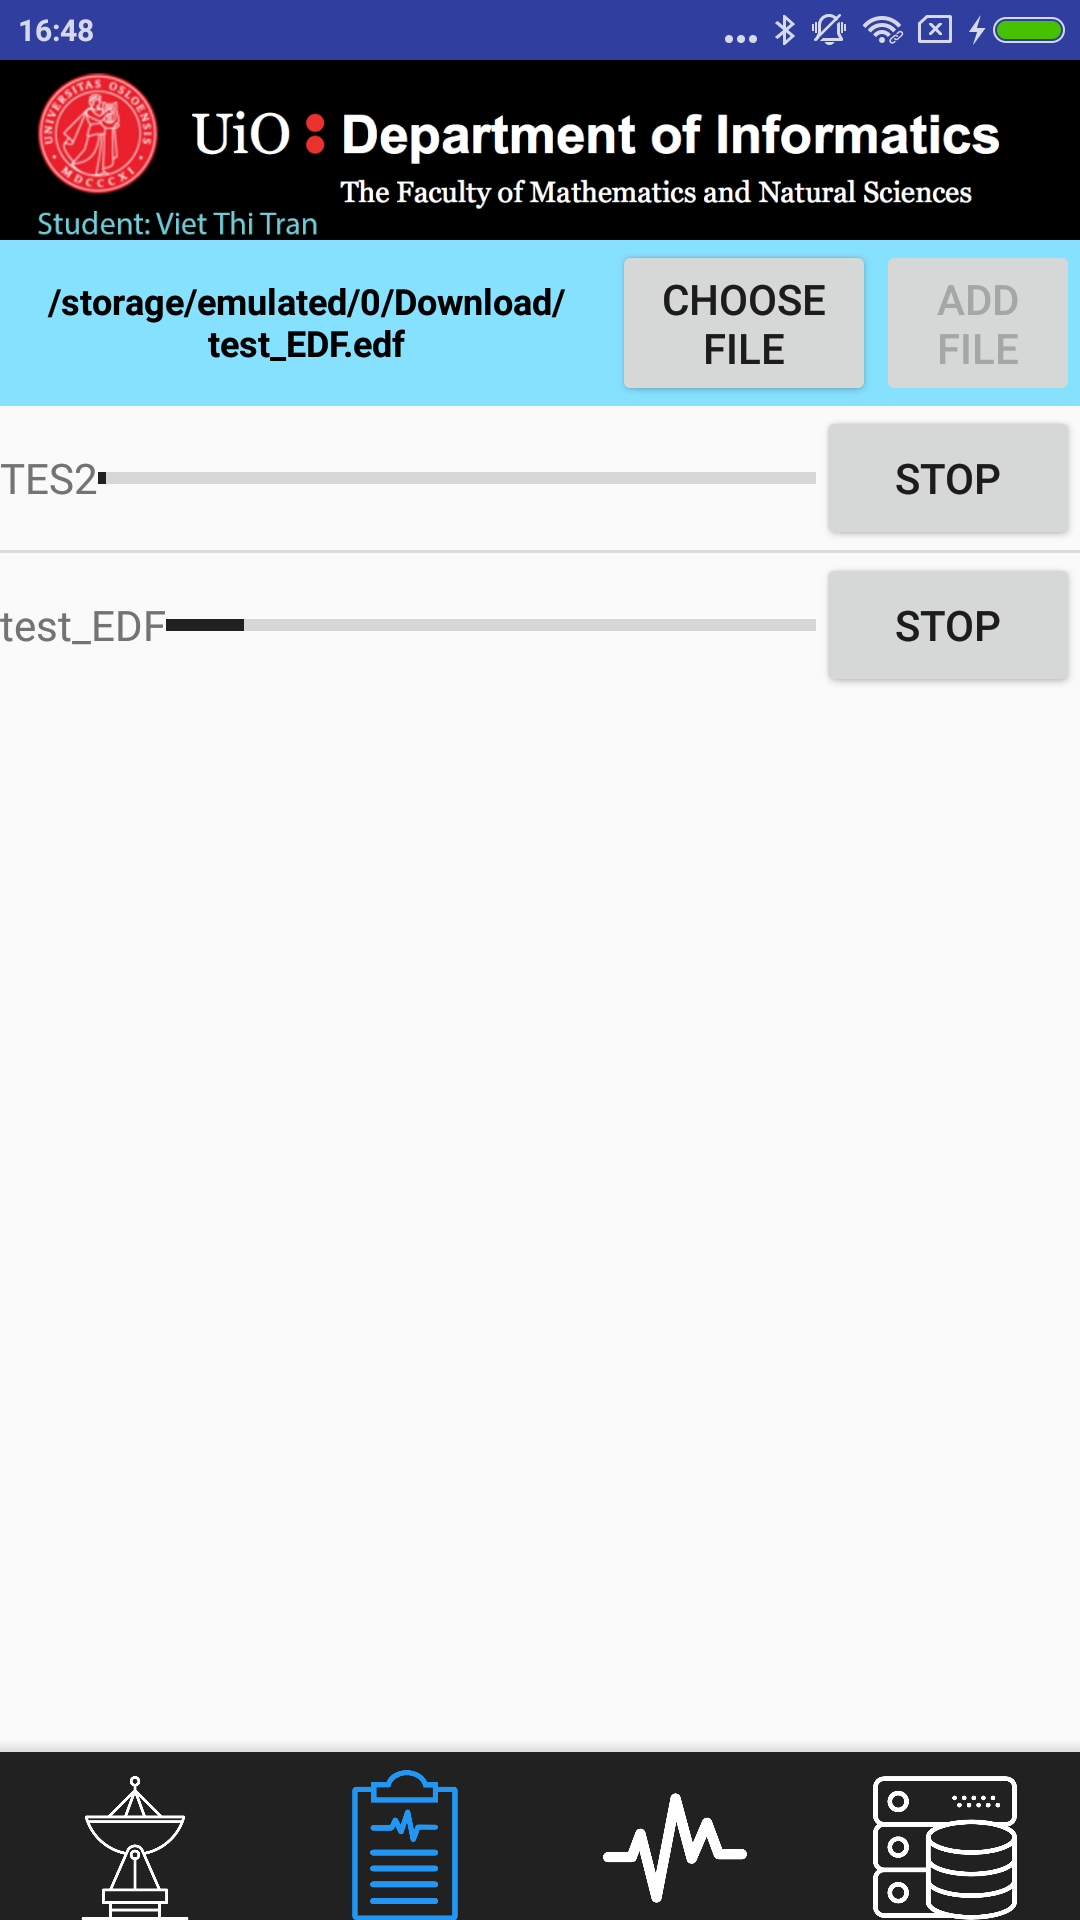
\includegraphics[width=60mm]{Figures/EDFimport.png}}
        \subfigure[EDF export GUI]{\label{fig:EDFexport}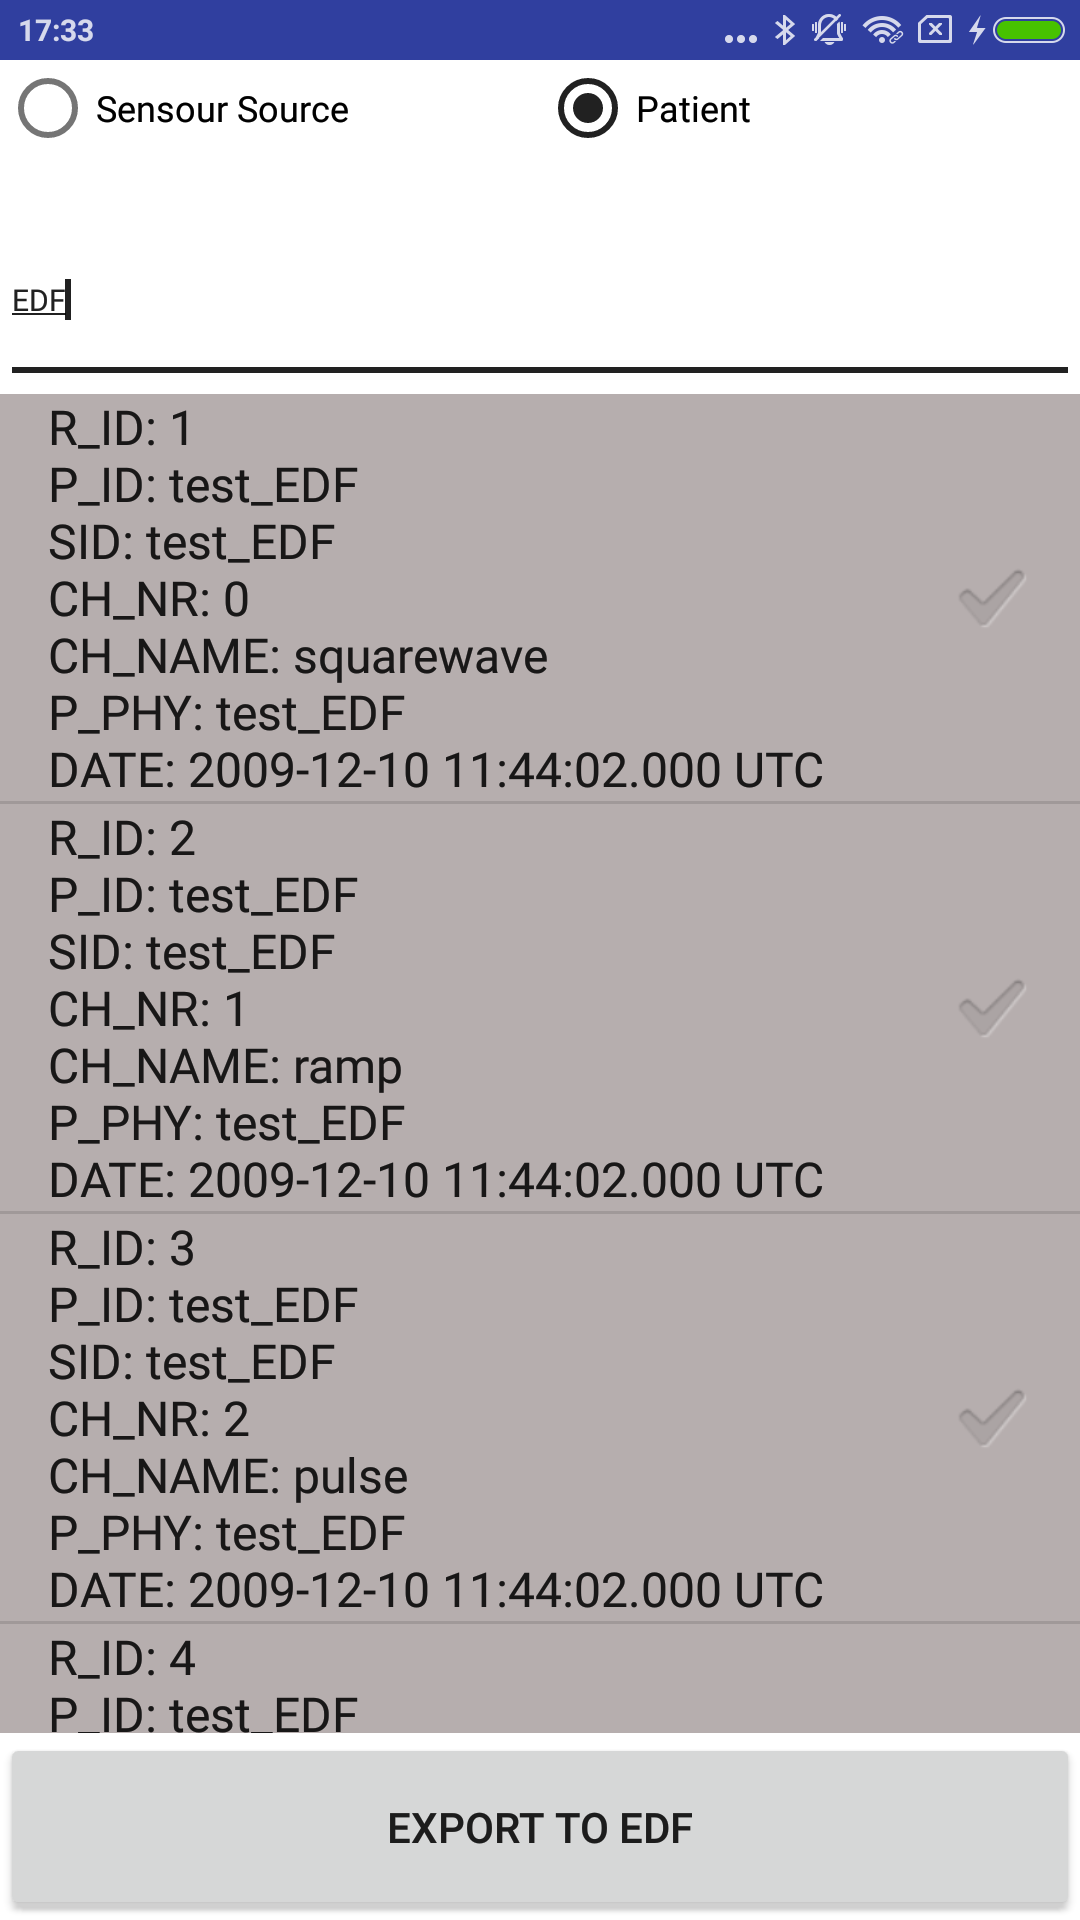
\includegraphics[width=60mm]{Figures/EDFexport.png}}
        \caption{EDF wrapper}
\end{figure}
The wrappers also allow users to export information in the database to EDF or EDF+ file formats. As Figure \ref{fig:EDFexport} presents, the users can search all records based on either their ids, or the source ids they used for collecting data. After that, the users can choose which records they want to export to the EDF file. Annotations are depended on records, therefore, all annotations are queried into a buffer before storing procedure for data records begins. As Figure \ref{fig:Figures/EDFExporter} in the high level design presents, samples are partially queried into a buffer before flushing to EDF file. While writing the data records, the number of sample in the record must be set to minus one. It is because if something wrong happened under writing, the EDF file is registered as invalid file. When all data records are written to the file, the header of the file need to be updated to valid the file. List \ref{listing:EDFWriter} presents an overview of the EDF exporting procedure.
\begin{code}[ht]
\begin{lstlisting}
public void run(){
    final String filePath = file_source.getFilePath();
    try {
        EDFHeader header = null;
        InputStream is = new BufferedInputStream(
                       new FileInputStream(new File(filePath)));
        //Parse Header to create new sensor source
        header = EDFHeaderParser.parseHeader(is);
        is.close();
        if (header == null) {
            sendMessageToHandler(FILE_IS_LOADED, file_source.getIndex());
            return;
        }
        createAndStoreSensorSource(header);
        createAndSavePatientPhysicianClinic(header);
        createAndSaveRecord(header);
        createAndStoreChannels(header);

        saveRecordFragmentAndSample(header);
    }catch (Exception e){
        e.printStackTrace();
    }
    sendMessageToHandler(FILE_IS_LOADED, file_source.getIndex());
}
\end{lstlisting}
\caption[EDF file reader]{EDF file reader}
\label{listing:EDFREADER}
\end{code}
\begin{code}[ht]
\begin{lstlisting}
public void run(){
    try{
        raf = new RandomAccessFile(this.fileName, "rw");
        buildEDFheader();
        storeDataRecord();
        //UPDATE TOTAL RECORD
        raf.seek(0);
        EDFWriter.writeEDFHeaderToFile(raf,edfHeader);
        raf.close();
    }catch (Exception e){
        e.printStackTrace();
    }
}
\end{lstlisting}
\caption[EDF file writer]{EDF file writer}
\label{listing:EDFWriter}
\end{code}
\subsection{Real-time and non-real-time visualization}
\begin{figure}
    \centering
    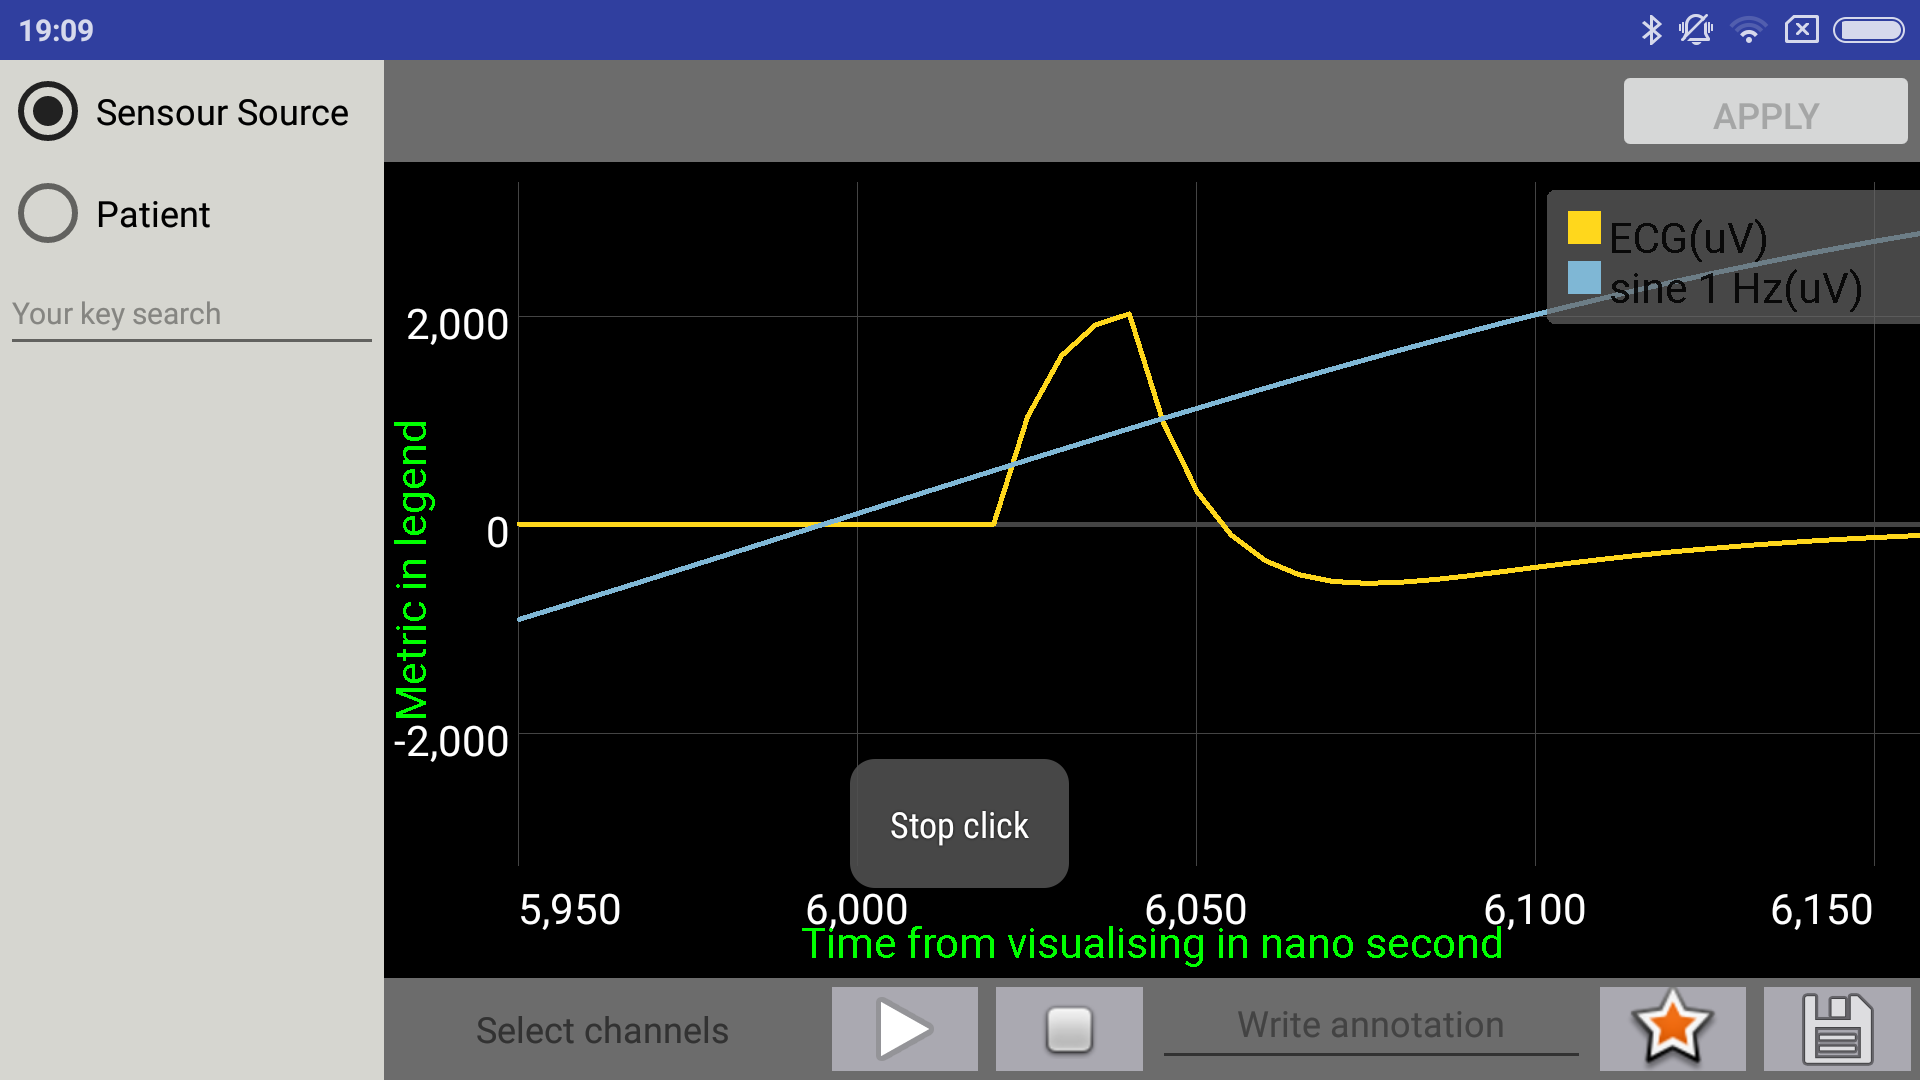
\includegraphics[width=0.9\textwidth]{Figures/NONPLOT.png}
    \caption{Replay samples from the database GUI}
    \label{fig:Figures/NONPLOT}
\end{figure}
For representing samples, a graphical technique is used in the implementation, that is a line-based plot. Each sample is presented in the graph with respect of time and its values. Arrival samples are updated to the graph dynamically. To avoid memory problem, the implementation does not keep all samples in the buffer for plotting. A sliding window buffer is used to keep the presented samples. That is, when the buffer is full, the oldest sample is replaced by the new arrival sample. The implementation uses an open source module, which is Android Graph View\cite{GRAPHVIEWMAIN} for presenting the samples. To solving dynamic plotting, the source also uses a sliding window to avoid memory leaks. That is, before adding a data point to the graph, the buffer is checked if it is full, and the oldest data point is removed in case the max count is reached. List \ref{listing:APPENDINTERFACE}\cite{GRAPHVIEW} presents the interface for appending new data points, and \ref{listing:PLOTGUI} presents how it is used in the implementation.\\
\begin{code}[ht]
\begin{lstlisting}
/**
 *
 * @param dataPoint values the values must be in the correct order!
 *      x-value has to be ASC. First the lowest x value and at least the highest x value.
 * @param scrollToEnd true => graphview will scroll to the end (maxX)
 * @param maxDataPoints if max data count is reached, the oldest data
 *                      value will be lost to avoid memory leaks
 * @param silent    set true to avoid rerender the graph
 */
public void appendData(E dataPoint, boolean scrollToEnd, int maxDataPoints, boolean silent);
\end{lstlisting}
\caption[appendData interface\cite{GRAPHVIEW}]{appendData interface\cite{GRAPHVIEW}}
\label{listing:APPENDINTERFACE}
\end{code}
In real-time visualization, the graph is passively waiting for other threads update its’ buffer, and notify it when the buffer is updated such that the graph can refresh the GUI. Non-real-time visualization, in contrast, has to query data from the database, and presents the queried data on the graph. A user, therefore, can pause and play queried samples at any moment in time. However, the user cannot do it in real-time visualization. It is because if the feature is supported, some samples do not have a chance to show in the graph. The feature is easily optimized in case the user wants to pause the plotting process in real-time, and the implementation for the visualization is a proof-of-concept, therefore it is not further discussed in detail in this subsection. Figure \ref{fig:Figures/NONPLOT} presents a GUI for non-real-time visualization, in which sources of data can be retrieved by searching the database based on either sensor source id, or patient id. By clicking on a source from the result list and applying it, the user can perform visualization process by interacting with play, pause, write annotation, select channels, save annotation components in the GUI.
\begin{code}[ht]
\begin{lstlisting}
v.post(new Runnable() {
    @Override
    public void run() {
        for(BitalinoDataSample sample: samples){
            LineGraphSeries<DataPoint> tmp = channelLines.get(sample.getChannel_nr());
            if(tmp != null && isReady)
                tmp.appendData(new DataPoint(channels.get(
                sample.getChannel_nr()).getLastXRealtime(),sample.getSample_data()),
                true,NR_ENTRIES_WINDOW);
        }
    }
});
\end{lstlisting}
\caption[Update samples to GUI]{Update samples to GUI}
\label{listing:PLOTGUI}
\end{code}